% Use a one-sided article template
\documentclass[oneside]{article}
% Decrease the margins a little
\usepackage{fullpage}

% Set up for including graphics
% We'll use png or pdf graphics
\usepackage[pdftex]{graphicx}
\DeclareGraphicsExtensions{.png,.pdf}

% Hyperref adds hyperlinks to the document automatically
% It's not much use yet, but it will be
\usepackage{hyperref}

% For including code into the document
\usepackage{verbatim}

% Tweak the default fonts a little
\renewcommand\rmdefault{bch}
\usepackage[small]{caption}
\usepackage[small]{titlesec}
\linespread{1.07} 

\raggedbottom
\pagestyle {empty}

\begin{document}

\begin{center}
\textbf{Stat640 - Progress Report 1 - Charlemagne and the Carolingian Empire (Delhey/Portman)}
\end{center}

\begin{center}
  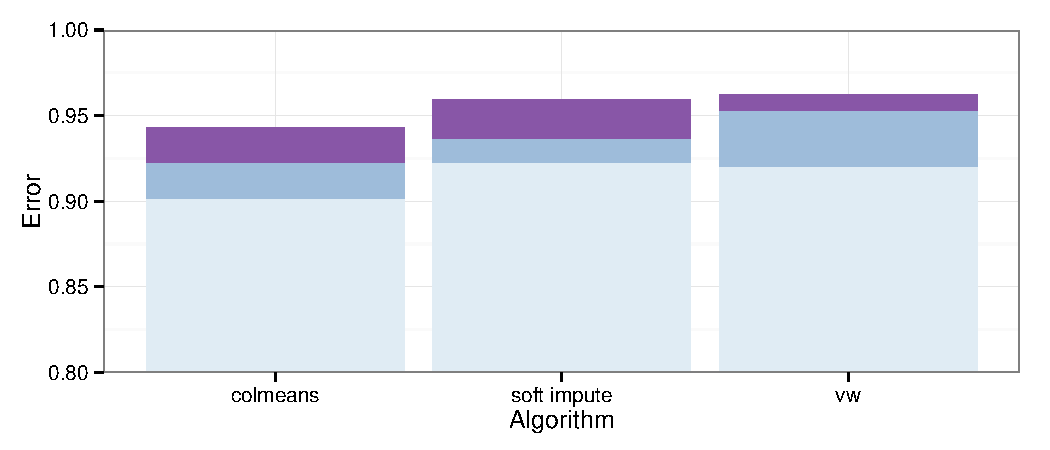
\includegraphics[width = 0.7\linewidth]{vis}
\end{center}

{\small
\begin{description}
\item[What learning algorithms have you tried?]
  \begin{itemize}

  \item \textbf{colmeans} The colmeans idea started with the provided benchmark, but we wanted some way to take in account individual users as well. We first accomplished this by subtracting the overall movie rating average (around 3.5) from the user's average movie rating and then adding this number to all the user's predicted ratings. This resulted in our highest performing algorithm. 

We then tried doing the same thing except instead of subtracting the overall movie rating average from the user's average, we subtracted only the rating average for movies that the user had rated. The idea was that this would account for the types of movies the user had rated which might not be representative of the entire set of movies and so would misrepresent the user's ratings relative to the average. The result of this formulation of colmeans actually performed the worst out of all of our submissions. We believe this is because the model overfit to the movies that the user had rated, i.e. the training data.

  \item \textbf{vow pal wabbit (vw)} One idea we had was to try linear regression. We converted the data set into a format that had one row for each rating and then joined the data with relevant user and movie columns. In this format the data was too large to run even a linear model in R on our local machines, so instead we used a program called \textit{vowpal wabbit}, a very fast linear learner. The predictions resulting form the algorithm seemed to overfit to the training data. Additionally, a linear model may not be an appropriate solution to such a collaborative filtering problem.

  \item \textbf{soft impute} We wanted to experiment with a method that makes heavy use of Singular Value Decomposition since the SVD gives you a low rank approximation of the decomposed matrix and helps break down the problem into a more palatable format. The 'softimpute' algorithm uses iterative soft-thresholded svds to impute the missing values.
  \end{itemize}

\item[Performance. Which algorithms worked well? Which performed poorly? Why?] The above graphic provides a summary of the performance of each method that we tried. The first bar represents the training error, the second bar represents the in-house testing error, and the final bar represents the leaderboard error. As stated, our implementation of colmeans has so far given us the best leaderboard error. We believe this is because it does a decent job of taking in account user preferences and movie tendencies through its high level aggregation. \textit{Vowpal wabbit} returned our worst leaderboard error due to overfitting of the training data. A naive implementation of the softImpute algorithm yielded pretty good results. However, we did not yet optimize the model parameters. This could potentially improve the model significantly.

\item[Project organization.] In order to deal with the inevitable technical problems of collaboration, our team has setup a github repository to share code and results. We've also both setup DAVinCI accounts and successfully ran jobs on the cluster. Looking forward, we are in the process of creating a shared folder on DAVinCI and plan on utilizing the cluster for future computations.

{\footnotesize
\item[Have you innovated? If so, how?] As of now we have not innovated in any interesting way. We believe that there is still a lot of performance we can squeeze out of more basic implementations.


\item[What are the future direction in which you would like to go?] Looking forward, we want to keep experimenting with novel algorithms and methods. We expect that our best performance at the end of the competition will result from an ensemble of models we have built in the interim and believe that such experimentation will pay off with a superior final model.
}

\end{description}

\end{document}